\documentclass{article}
\usepackage[utf8]{inputenc}
\usepackage[a4paper, total={6in, 8in}]{geometry}
\usepackage{xcolor}
\usepackage{graphicx}
\usepackage[font=small,labelfont=bf]{caption}
\usepackage{ulem}
\usepackage[hyphens]{url}
\graphicspath{ {./images/} }
\newcommand{\tabitem}{~~\llap{\textbullet}~~}
\usepackage{multicol}
\usepackage{titlesec}
\usepackage[super]{natbib}

\newenvironment{Figure}
  {\par\medskip\noindent\minipage{\linewidth}}
  {\endminipage\par\medskip}

% \counterwithin*{equation}{subsection}
% \renewcommand{\theequation}{\arabic{section}.\arabic{subsection}.\arabic{equation}}
% \setlength{\parskip}{6pt}

% \titlespacing{\section}{12pt}{\parskip}{-\parskip}
% \titlespacing{\subsection}{12pt}{\parskip}{-\parskip}

\usepackage{hyperref}
\usepackage{amsmath}
\usepackage{subcaption}
\usepackage{float}


\title{Simulating the Radio Sky for the DSA-2000}
\author{Tyrone McNichols \\Mentors: Gregg Hallinan, Yuping Huang, Casey Law}
\date{}



\begin{document}

\maketitle

\begin{abstract}
    The Radio Camera Initiative (RCI) has put forth a new approach to radio telescopes called the radio camera which is able to directly output science-ready image data to the end user rather than the normal visibilities. This approach bypasses the need for deconvolving the point source function of the instrument, a particularly expensive computation. As a result, this greatly increases the rate at which data products are produced and thus the potential scientific return of the telescope. The 2000-antenna Deep Synoptic Array (DSA-2000) is a proposed radio telescope that will pioneer this approach. In order to bring the radio camera concept to life, there are new calibration and engineering requirements that must be addressed in the design phase. In this project, I address two key aspects in the DSA-2000's development: survey strategy design and instrument simulation. The survey strategy is expressed as an optimization problem, and a framework for solving this problem and adding additional constraints is presented. For instrument simulations, model sky data is necessary to test the efficacy of the data pipeline and imaging algorithms. True sky images for such purposes are constructed using catalogs of bright radio sources from previous sky surveys and catalogs of active galactic nuclei (AGNs) and star forming galaxies (SFGs) generated with the Tiered Radio Extragalactic Continuum Simulation (T-RECS).
\end{abstract}

\begin{multicols*}{2}

\section{Introduction}

Presently, there is a large bottleneck in radio astronomy limiting the potential scientific output of radio interferometers. The main data product of an interferometer is the complex visibility which is the Fourier transform of the sky brightness distribution. An interferometer is capable of producing sampled visibilities for every pair of apertures in the array per frequency channel per cross-polarization, so as the number of apertures $n$ in the array increases, the number of visibilities produced increases like $n(n-1)/2$. Thus, as the size of interferometers has increased with time, the amount of data served to the end user has likewise increased. Modern radio interferometers typically deliver the visibilities to end users via a public archive, who are then responsible for converting the data into scientific images using a variety of software packages. This process requires the user to i) identify and remove (flag) bad data, ii) calibrate the relative phase and amplitude of the signal at each antenna and iii) interpolate the visibilities on to a uniform grid, which in turn enables the use of a 2-D FFT to produce an image. \cite{dsa2000} However the resulting image is typically initially unusable for science. This is because the limited number of antenna in most modern radio interferometers results in a very poor point source function (PSF), resulting in sidelobes that dominate the noise in the resulting images. The resulting ``dirty image'' (Figure \ref{fig:dirty_image}) is the convolution of the true sky brightness and the PSF of the instrument. To recover the true sky brightness, the deconvolution of the image must be computed, which is computationally expensive with current methods such as the CLEAN\cite{Hgbom1974APERTURESW} algorithm. With increasing data volumes and rapidly aging tools for data reduction, the computational burden on the end-user has grown rapidly in the past few decades and is showing no signs of slowing down.


\begin{figure*}
    \centering
        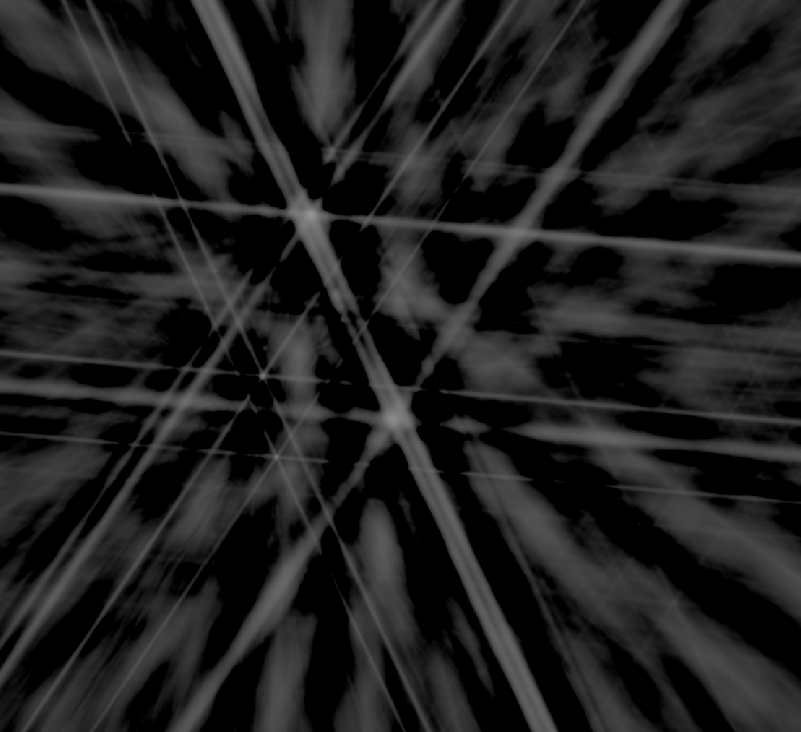
\includegraphics[height=0.4\linewidth]{images/dirty VLASS.png}
        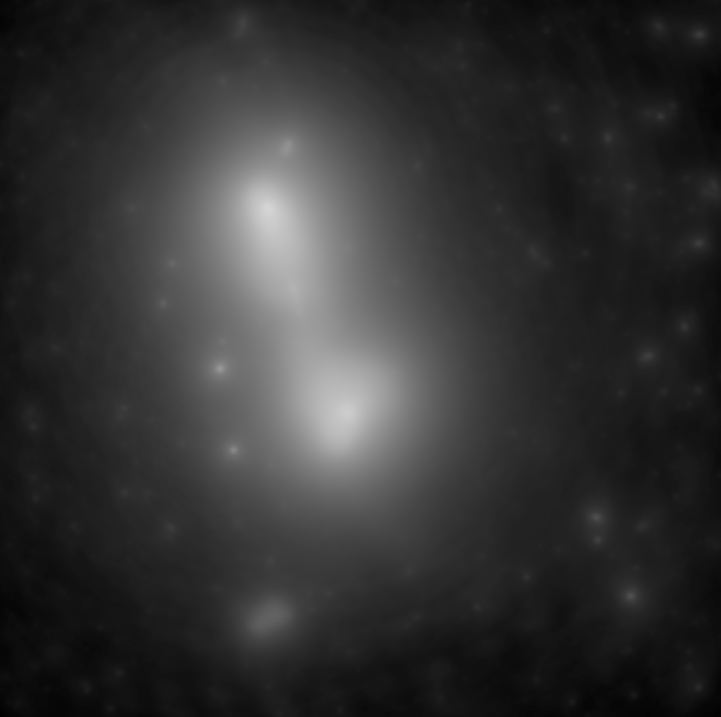
\includegraphics[height=0.4\linewidth]{images/dirty DSA.png}
    \caption{Two example ``dirty images'' of the same region of the sky. The left image, simulating the Very Large Array Sky Survey (VLASS) \cite{Lacy_2020}, shows much more pronounced sidelobe artifacts than the right image, a simulated image from the DSA-2000. The DSA-2000 is able to achieve this better image due to its improved PSF over the VLA.}
    \label{fig:dirty_image}
\end{figure*}

The Radio Camera Initiative (RCI) seeks to resolve this problem by constructing an interferometer that achieves a good enough PSF such that deconvolution becomes unnecessary (see Figure \ref{fig:dirty_image}). Such a machine has been dubbed a ``radio camera'', as it would be capable of producing science-ready images in real time rather than the normal visibilities \cite{dsa2000}. To pioneer this new approach, the RCI has proposed The 2000-antenna Deep Synoptic Array (DSA-2000). The DSA-2000 will use an integrated backend that will produce visibilities, flag bad data, calibrate the array, and produce a final science-ready image in real-time \cite{dsa2000}. Thus far, work has been done on developing this backend and simulating the instrument.

In this project, I work on two major aspects of the development of the DSA-2000: i) survey strategy development and ii) the construction of model sky data for instrument simulations. For a radio camera like the DSA-2000 that has to calibrate the array in real time, it is imperative that the imaging process is as easy  as possible. As a result, the survey strategy developed attempts to find a collection of antenna pointings that minimize the imaging difficulty. To this end, the strategy is expressed as an computational optimization problem. I then create a framework for solving this problem using integer linear programming (ILP). The model sky data is created to serve as a reference ``true sky'' in instrument simulations. With this data as a reference, the efficacy of algorithms developed for the backend and configurations of the array can be properly evaluated. The data itself is in the form of a Flexible Image Transport System (FITS) image representing what the DSA-2000 may actually observe. The data in the FITS image come from a collection of catalogs containing source information such as source size and flux density.




\section{Methods}
\subsection{Survey Strategy}

\begin{figure*}
    \centering
    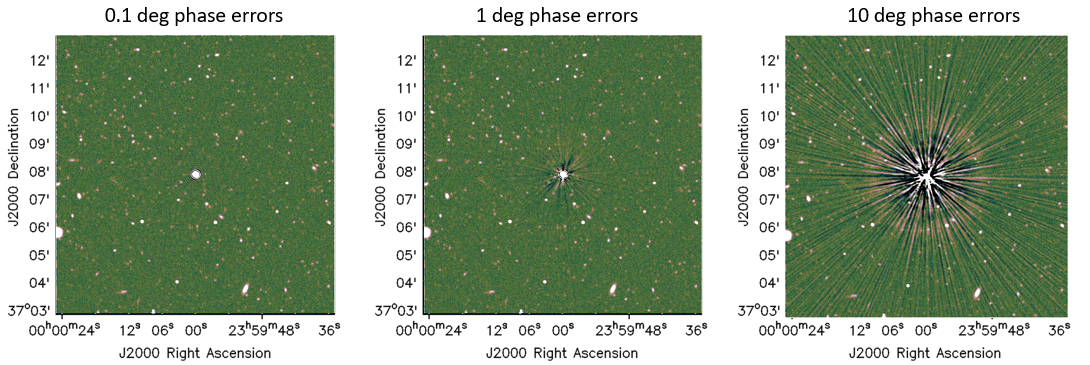
\includegraphics[scale=0.5]{images/artifacts.png}
    \caption{Examples of simulated data for 0.25\% of the field-of-view of the DSA-2000. The sky model from SKA Data Challenge \#1\cite{skadata1} serves as the initial ``True Sky'' with the image centered on the brightest source in the $\sim$7 square degree image. The observation simulated is for a single 15-minute integration. The image shows the results after image-plane CLEAN for residual direction-independent phase errors of 0.1°, 1° and 10° (left to right).}
    \label{fig:artifacts}
\end{figure*}

When defining a survey strategy for the DSA-2000, I focus on finding the best way to map the sky while also taking into account the unique properties of the DSA-2000. Ideally, a sky survey will map the entire sky region with uniform sensitivity. This ensures that the survey will be able to recover potential radio sources near the sensitivity limit in all regions of the sky. Usually, surveys will opt for a simple way to tile the sky, such as uniformly splitting the region into squares the size of the field-of-view of the telescope. However, such a strategy is ill-suited for a radio camera such as the DSA-2000. The DSA-2000 must be able to take visibilities and convert them to science-ready images in real time. One major obstacle to real-time imaging is the presence of bright radio sources. I classify bright sources as those with peak flux density greater than 100 mJy based on the 99\textsuperscript{th} percentile of peak flux density in the the Very Large Array (VLA) Faint Images of the Radio Sky at Twenty-Centimeters (FIRST) Sky Survey \cite{FIRST} data catalog. The reason bright sources make real-time imaging difficult is two fold. Firstly, bright sources make calibration harder since the calibration sky model needs to account for each source. Secondly, bright sources introduce pronounced artifacts into the image which get worse with increasing gain-phase errors. Furthermore, bright sources have bright sidelobes which lead to higher gain artifacts. Figure \ref{fig:artifacts} shows an example of such artifacts of bright sources and how they change with increasing gain-phase errors.

As a result, for the DSA-2000, an optimal survey strategy is one that not only achieves uniform sensitivity, but also minimizes difficulties caused by bright sources. The sensitivity of the telescope is highest in the center of primary beam of the antenna's response, so ideally the entire sky would be mapped within the primary beam. Keeping mapping within the full width at half maximum (FWHM) of the primary beam of the telescope (for the DSA-2000 this is approximately 2.2 deg) would allow for near uniform sensitivity while also maximizing the overall sensitivity of the survey. Bright source artifacts can be minimized by keeping bright sources as close to the center of the primary beam in any given pointing, as phase errors increase with distance from the center of the primary beam of the telescope. Similarly, keeping few bright sources in a pointing would  help alleviate calibration difficulties.

Next, I formulate this survey strategy as a
computational problem. In this formulation, I
treat the sky region being mapped as a discrete
grid $T$ of $n$ tiles, along with a set $S$ of bright sources in the sky region. The tiles represent potential centers of antenna pointings, each with their own imaging-difficulty cost associated with them due to the bright sources in $S$. For every tile $t$, a pointing includes every tile and
every source within a circle with diameter equal
to the FWHM of the primary beam. This collection
of tiles is called the neighborhood of $t$, $N(t)$, and the collection of bright sources is called $B(t)$, both of which are formally defined as
\begin{align}
    N(t) &= \left\{a \in T \mid d(a,t) \leq \mbox{FWHM}/2 \right\}\\
    B(t) &= \left\{s \in S \mid d(s,t) \leq \mbox{FWHM}/2 \right\},
    \label{eq:neighborhood}
\end{align}
where $d$ is the angular distance. 

Every bright source $s \in B(t)$ contributes to the cost $c(t)$. The cost from each source is the product of the angular distance to the tile $t$ and the peak flux density of the source $f(s)$ giving the total cost of $t$:
\begin{equation}
    c(t) = \sum_{s \in B(t)} d(s,t) \cdot f(s).
    \label{eq:cost}
\end{equation}
This cost function incentivizes bright sources being as close to the center of a pointing as possible. Moreover, the function incentivizes having few bright sources in the pointing, as having zero bright sources would reduce the cost to 0. These two properties are precisely what is desired.

Finding the optimal survey strategy then becomes finding a subset $U \subseteq T$ such that every tile is in the neighborhood of some tile in $U$ (tiling the sky with the FWHM) and the total cost of $U$ is minimized (minimizing bright source difficulty). More formally, given the sets of tiles and bright sources $T$ and $S$, find a subset $U \subseteq T$ such that 
\begin{align*}
    &\forall\ t \in T,\ \exists\ u \in U\ \mbox{such that}\ t \in N(u)\\
    &\mbox{and}\ \sum_{u \in U} c(u)\ \mbox{is minimized}.
\end{align*}

To implement an algorithm solving this optimization problem, I create an ILP as the problem lends itself nicely to the approach. The linear program is written in the form:

\begin{equation}
    \label{eq:lp}
    \begin{array}{cc}
        \mbox{minimize} & c^\dagger x\\
        \mbox{s.t.} & Ax \geq b\\
         & x_i \in \left\{0, 1 \right\} \forall\  1 \leq i \leq n,
    \end{array}
\end{equation}

where $n$ is the number of tiles, $c$ is an $n$ dimensional vector containing the cost of each tile, $x$ is an $n$ dimensional vector representing which tiles are chosen as centers of pointings, $A$ is an $n \times n$ matrix encoding $N(t)$ for every tile $t$, and $b$ is an $n$ dimensional vector full of just 1. The entries in $x$ are either 1 or 0, a 1 in position $i$ indicating that tile $t_i$ is a chosen center of a pointing. Every entry in $A$ is either 1 or 0, with a 1 at $a_{ij}$ indicating that $t_i \in N(t_j)$. $Ax$ will have in each position $i$ of the resulting vector  the number of times tile $t_i$ is in a pointing. So enforcing $Ax \geq b$ is equivalent to saying each tile is included in at least one pointing, i.e the sky is tiled by the pointings.

To actually solve the ILP, the costs of the tiles are calculated and given as inputs to PuLP\cite{pulp} which employs a number of algorithms to solve linear programs. For the set of bright sources in the sky, the VLA FIRST Sky Survey data catalog is used. The program, when run, outputs which tiles are optimal for antenna pointings. Figure \ref{fig:survey_example} shows an example output with sources from the VLA FIRST Sky Survey in the region 195-205 deg right ascension (RA), 20-30 deg declination (DEC). The green circles represent the individual pointings, with diameter equal to 2.2 deg, the FWHM of the primary beam of the DSA-2000.

\begin{figure*}
    \centering
    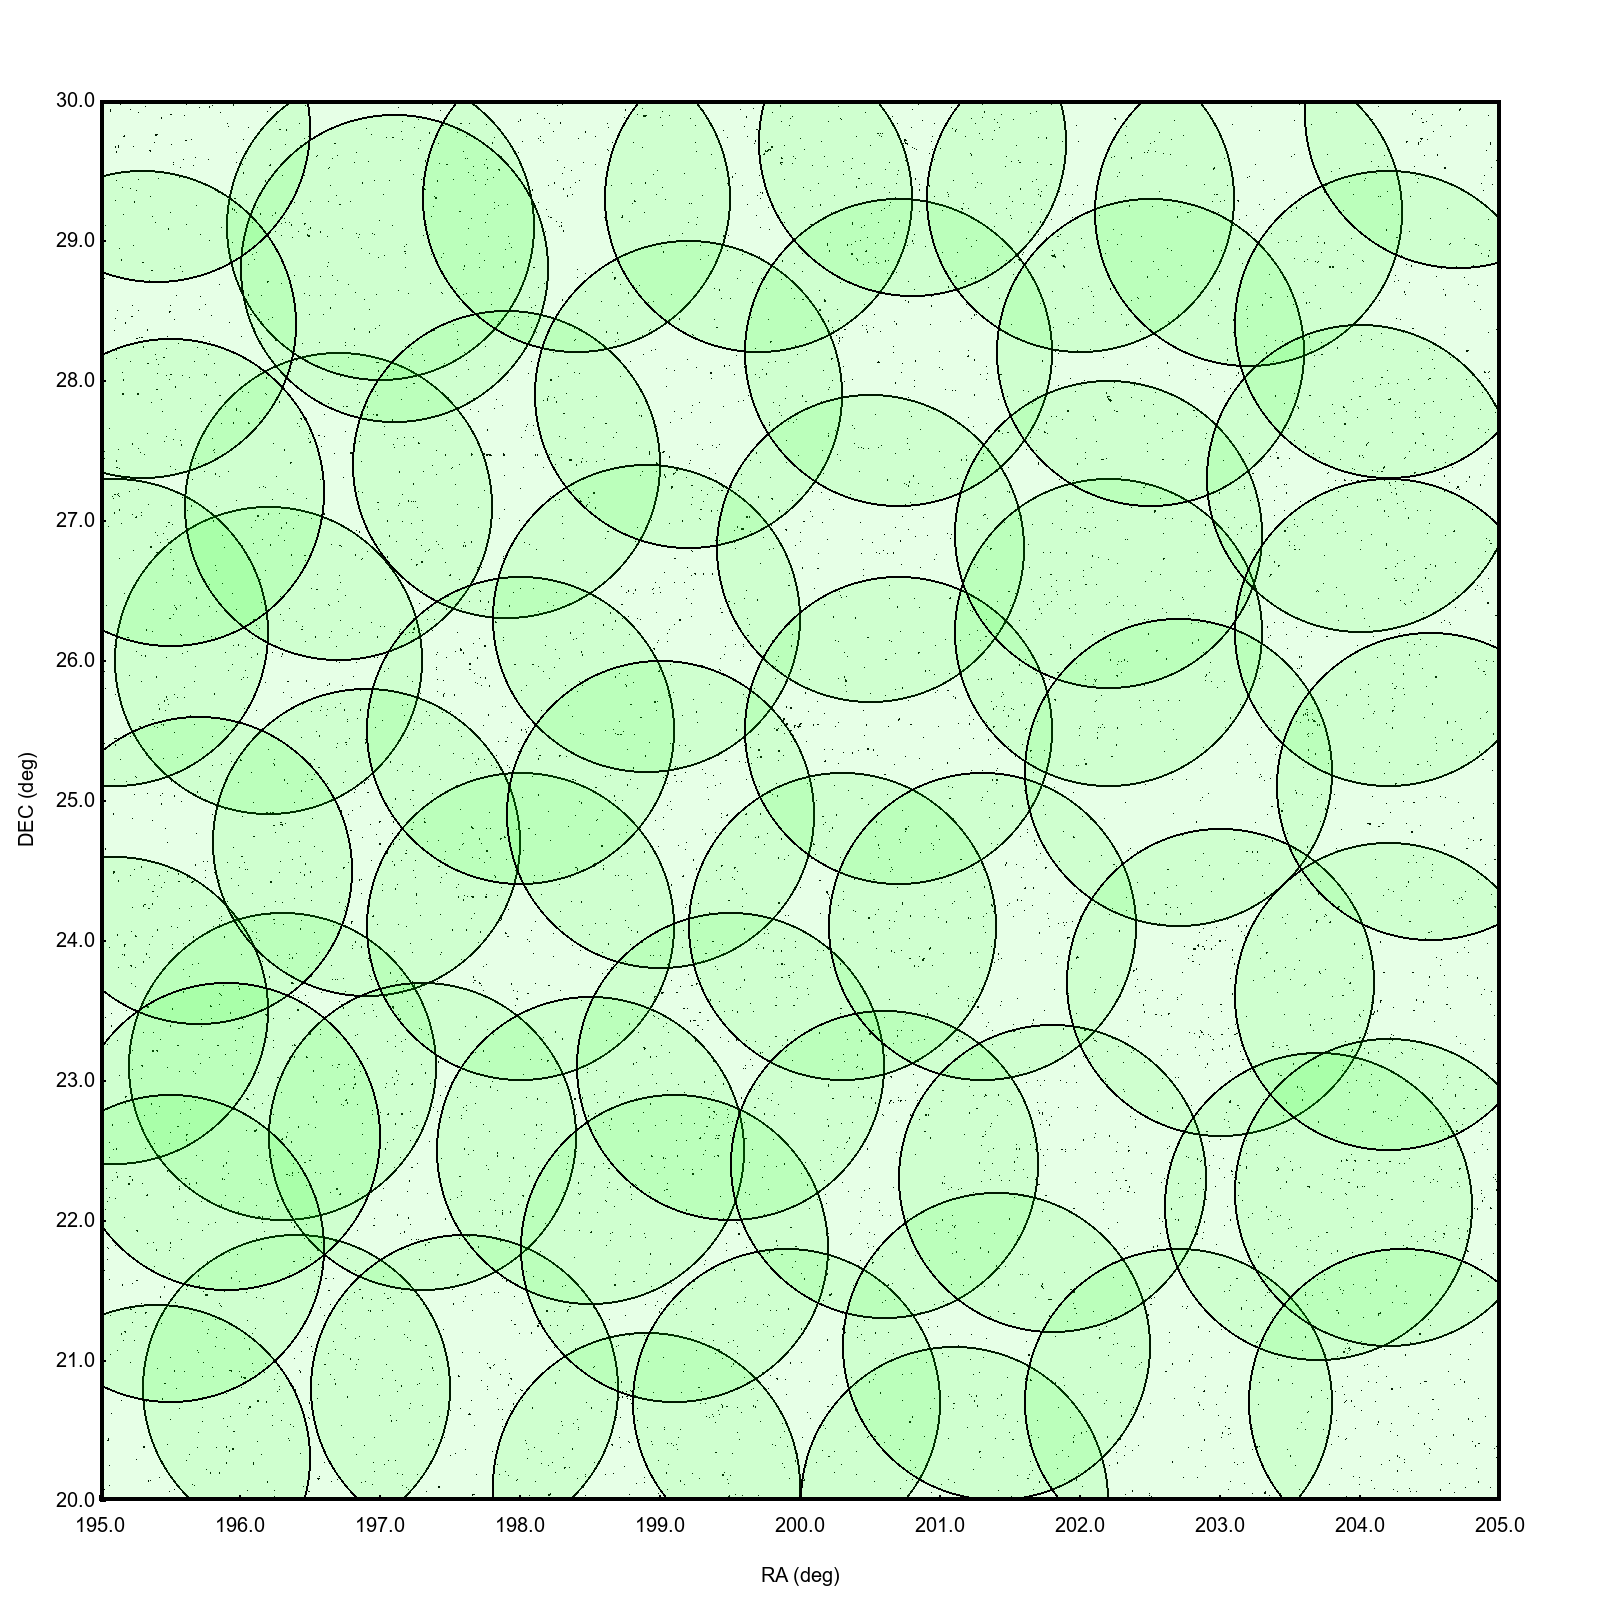
\includegraphics[width=\textwidth]{images/20_195_to_30_205.PNG}
    \caption{Example output of survey strategy optimization. The green circles represent the FWHM of the primary beam of the DSA-2000. The sources used, visualized with the black points in the image, were the bright sources from the VLA FIRST Sky Survey in the region 195-205 deg RA, 20-30 deg DEC. This optimization was done with a tile size of $0.1\times0.1\ \mbox{deg}^2$ for a total of 10000 tiles in the region.}
    \label{fig:survey_example}
\end{figure*}

\subsection{Model Sky Data}

For the model sky data, it is important that it accurately represents what the DSA-2000 may actually see during observations. Furthermore, as bright radio sources present a unique challenge to the array, it is important to include such sources in the model. To that end, the data is created by combining catalogs of sources of varying flux densities, redshifts, and morphologies. For bright sources, I use the VLA FIRST Sky Survey catalog, which contains 946,000 sources above a 1 mJy detection threshold over 10,000 square degrees. To model dimmer sources, the Tiered Radio Extragalactic Continuum Simulation (T-RECS) \cite{trecs} is used to generate two catalogs of sources: one containing 241192 star forming galaxies (SFGs) and one containing 31556 active galactic nuclei (AGNs). The AGNs are further delineated into 21277 steep spectrum AGNs (SSAGNs), and 10279 flat spectrum AGNs (FSAGNs).

These catalogs are generated for a $5\times 5\ \mbox{deg}^2$ region of the sky centered at 0 deg RA and 0 deg DEC. The redshifts $z$ of the sources range from $z=0$ to $z=8$. The specific size of the sky region and the redshift bounds are chosen because they are the maximum that still permit dark matter halo clustering with T-RECS, an important feature to ensure accuracy of the model. As the sensitivity of the DSA-2000 is 1 $\mu$Jy, all sources are generated with that as the flux limit. All source flux densities are generated at 1350 MHz, the center of the frequency coverage of the DSA-2000. 

The radio sources from the three catalogs were then added to a FITS image as elliptical Gaussian components. The final image is $8192 \times 8192$ pixels yielding a resolution of about 2.2 arcsec / px.

The sources from the VLA FIRST catalog and the SFG catalog are described by the peak flux density $f$, a major and minor axis ($a,b$), and a position angle $\phi$. Since the SFG catalog does not list major or minor axis or position angle, these values are derived from the two ellipticity components ($e_1, e_2$) and the size ($s$) using the equations:
\begin{equation}
    e = \sqrt{e_1^2 + e_2^2}, \label{eq:ellipticity}
\end{equation}
\begin{equation}
    a = \frac{s}{1 - e},
\end{equation}
\begin{equation}
    b = \frac{s}{1 + e},
\end{equation}
\begin{equation}
    \phi = \arctan\left(\frac{e_1}{e_2}\right). \label{eq:posang}
\end{equation}
The sources are approximated with an elliptical Gaussian with FWHM ($w_1, w_2$) in each dimension equal to half the axis length (i.e. $w_1 = a/2, w_2 = b/2$), yielding a full characterization of $(f, \phi, w_1, w_2)$.

FSAGNs are described by an integrated flux density $I$, a size $s$ (the largest angular size (LAS) of the source), and a core fraction $r_c$. The sources are approximated with a pair of circular Gaussians: a compact core with flux density $I_c \times r_c$, and FWHM of $w_c = 2.2$ arcsec, the pixel resolution of the image; and a more extended, end-on lobe with flux density $I_d = I * (1-r_c)$ and FWHM $w_d = s/2$. This yields the full characterization $(I_c, w_c), (I_d, w_d)$.

SSAGNs are not included in this initial data. This is because their morphologies are not easily captured with the elliptical Gaussian model that I used.

The final FITS image is shown in Figure \ref{fig:fits}.

\begin{figure*}
    \centering
    \includegraphics[width=\textwidth]{images/fits.png}
    \caption{Model sky data FITS image. This image contains the 2280 sources from the VLA FIRST Sky Survey in the region from -2.5 to 2.5 RA and DEC, as well as 241192 SFGs and 10279 FSAGNs from the T-RECS catalogs.}
    \label{fig:fits}
\end{figure*}

\section{Discussion}

\begin{figure*}
    \centering
    \begin{subfigure}{0.45\textwidth}
        \centering
        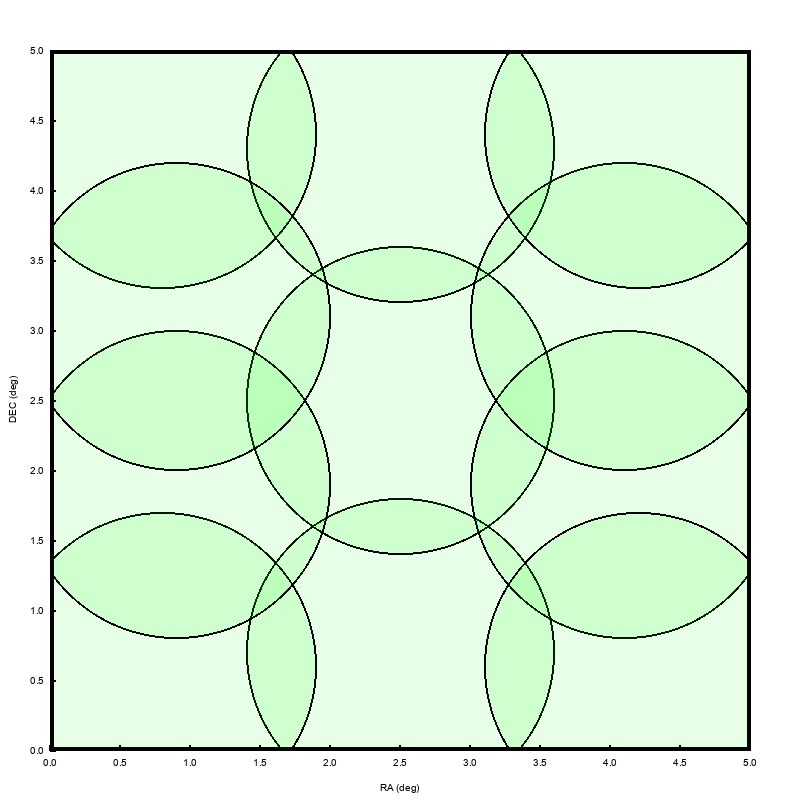
\includegraphics[width=\linewidth]{images/uniform.png}
        \caption{Optimal}
        \label{fig:empty_field1}
    \end{subfigure}
    \begin{subfigure}{0.45\textwidth}
        \centering
        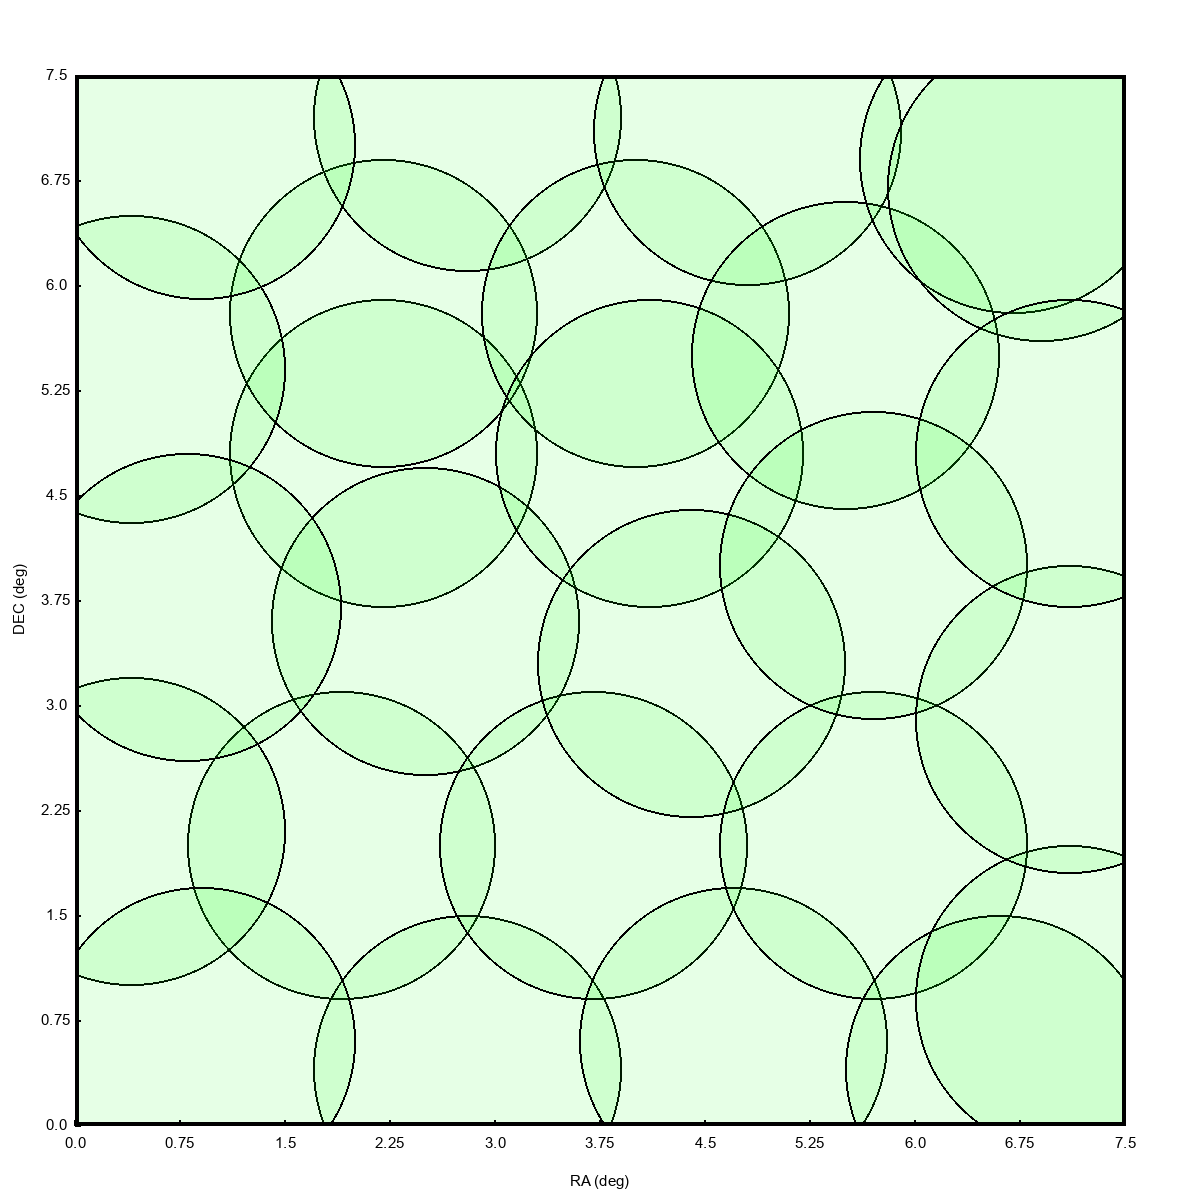
\includegraphics[width=\linewidth]{images/empty_field_suboptimal.PNG}
        \caption{Suboptimal}
        \label{fig:empty_field2}
    \end{subfigure}
    \caption{Results of sky survey optimization for a sky region with no bright sources. The left image shows the optimal results recovered for a $5\times 5\ \mbox{deg}^2$. Note that the circles are, as expected, arranged in a hexagonal pattern. The right image shows a suboptimal result obtained via a timeout.}
    \label{fig:empty_field}
\end{figure*}

\subsection{Survey Strategy}
The two main objectives for the survey strategy in this project were 1) to achieve uniform sensitivity, and 2) to minimize the real-time imaging difficulty. As a sanity test for uniform sensitivity, I verified that the ILP tiles the sky with the FWHM of the DSA-2000. As shown in Figure \ref{fig:survey_example}, the selected pointings (visualized with the green circles) tile the sky region, indicating that objective 1 is indeed satisfied.

While the output is definitely optimal based on the inputs that are given, it's worth questioning whether the ILP formulation does what is desired, i.e. does this program actually minimize imaging difficulty. To test this, I ran the program with specific sets of bright sources and compared with the expected results. For example, I ran the program with a sky region containing zero bright sources. In such a case, as there are no bright sources to account for, the problem reduces to finding an optimal way to tile the sky with as few pointings as possible. With such an input, one would expect the program to recover a regular tiling pattern. As shown in Figure \ref{fig:empty_field1}, the result was exactly what was expected: the program recovered a hexagonal tiling. This result is particularly interesting, as this is one of the tilings typically used for other surveys. A similar test was conducted by placing a few bright sources in specific locations such that the optimal results would be to place a pointing directly on each source, and this too was recovered by the algorithm. Thus, it is evident that the ILP is working as intended.

Although the current framework is working as intended, there are some limitations that should be addressed should this be explored more in depth in the future.

Perhaps the most important issue is that solving ILPs is known to be NP-Hard. As a result, as the size of the input increases (in this case $n$, the number of tiles), the speed of the program drastically decreases. As such, this algorithm is not efficient for running the program with larger regions of the sky. Similarly, if you keep the size of the sky region the same, but decrease the size of the tiles, you would increase the accuracy of the discrete approximation, however the program would take drastically longer to compute. One way I worked around this was by using linear programming (LP) relaxation. While solving ILPs is NP-Hard,  solving LPs without the integer restriction is solvable in polynomial time. This lends a natural way to approximate solutions to ILPs: solve the continuous version of the ILP, and then round the results to the nearest integer to gain an approximate solution to the ILP. To find the optimal solution to the ILP, one simply needs to find which way to round the LP solution. A common method for finding this rounding is by using branch and bound. Branch and bound works by searching a rooted tree containing all the possible solutions to the problem. The algorithm explores branches of this tree and is able to discard branches by checking them against estimated bounds of the optimal solution, reducing the amount of solutions to check and drastically reducing the runtime. By using branch and bound, this rounding approach can potentially find the optimal solution to the ILP much faster than normal algorithms would, however in the worse case it will still take exponential time as the entire tree will have to be searched. My workaround to this problem was to add a timeout on the branch and bound step. After some fixed amount of time, if the optimal solution hasn't been found yet, the most optimal ILP solution found so far will be accepted. An example of this can be seen in Figure \ref{fig:empty_field2}. This example was run with an empty field, so a regular tiling was expected. However, such a solution was not recovered in time, so the best solution found was output. By examining the distribution of pointings in the lower half of the sky region, one can see that the program was beginning to converge on a regular tiling. Another approach to this problem could be to find another algorithm to solve the problem. I opted for ILP initially, but 
\begin{figure}[H]
    \centering
    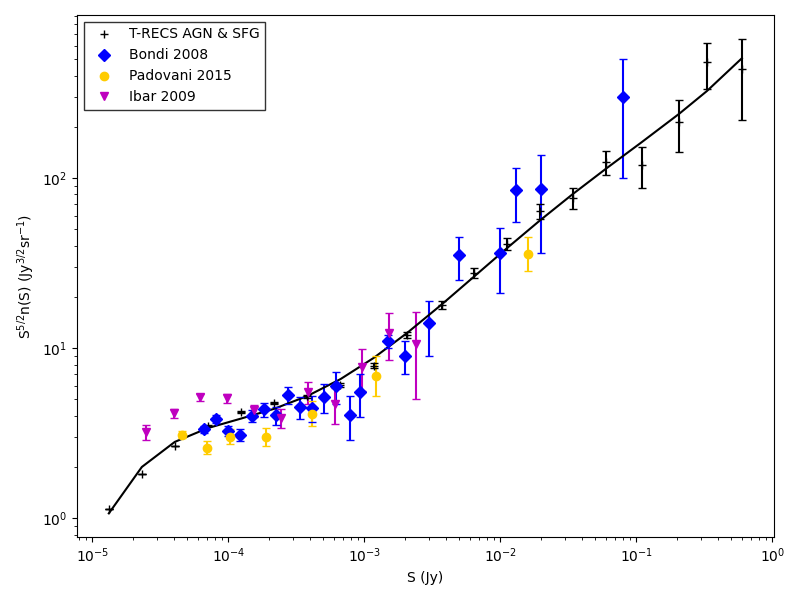
\includegraphics[width=\linewidth]{images/differential_src_counts.png}
    \caption{Comparison of normalized differential source counts in total intensity at 1.4 GHz between T-RECS AGN and SFG catalogs and the available data from \citet{Bondi_2008,Padovani_2015,Ibar_2009}.}
    \label{fig:counts}
\end{figure}
\begin{figure}[H]
    \centering
    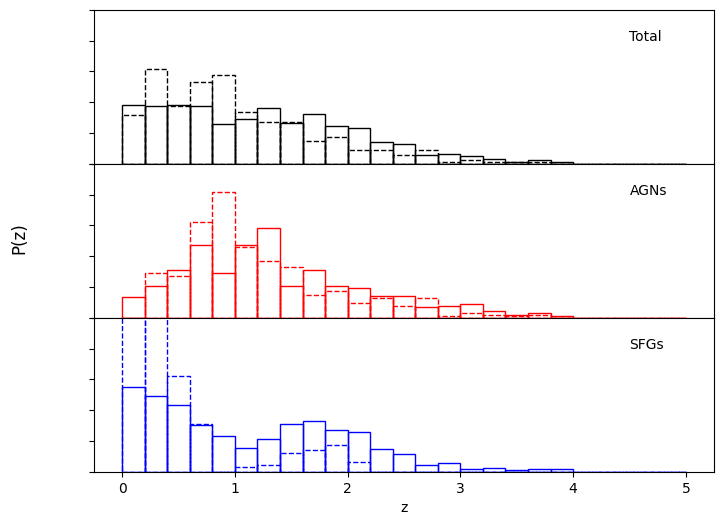
\includegraphics[width=\linewidth]{images/redshift.png}
    \caption{Comparison of the redshift distributions between \citet{10.1093/mnras/stw2541} (dashed lines) and the T-RECS catalogs (solid lines).}
    \label{fig:redshift}
\end{figure}
\noindent
it's quite possible there is another way to frame the problem that allows for faster solutions. One idea is using a greedy approach. Greedy algorithms can often provide fast solutions to problems that otherwise seem hard by using heuristics. Such a heuristic could be something like centering the next pointing on the brightest source that hasn't been included in a pointing yet. Of course, it would need to be proven that such a heuristic would guarantee an optimal solution.

The other major working point for the framework I laid out is the function used to calculate the cost for each tile. Although Equation \ref{eq:cost} does incentivize placing bright sources near the center of the primary beam, the direct linear relationship seems too simple to accurately portray the effects of bright sources. A more accurate model is needed to improve the accuracy of these simulations. Furthermore, Equation \ref{eq:cost} only takes into account the bright sources that are within the FWHM of the primary beam, however effects of bright sources can still be felt farther away. In fact, bright sources in the far sidelobes of the antenna present some of the largest challenges to calibration. As such the cost function must be updated to account for this.

As it stands, the survey strategy framework I have laid out is a proof of concept. While there are some noted limitations, the ideas behind the formalization of the problem seem to have carried through to the end product. Presently, the program does create a set of pointings that gets near uniform sensitivity while imaging calibration difficulty to some capacity. With a few changes to the cost calculation, and perhaps some reframing of the problem, this framework could be used when actually designing the DSA-2000's sky surveys.

\subsection{Model Sky Data}

I devised 2 tests to ensure that the source catalogs, specifically the AGN and SFG catalogs created with T-RECS, provided realistic source distributions for AGNs and SFGs.

First, I compared the differential source counts in the catalogs to that of the available data. Figure \ref{fig:counts} presents the comparison between the AGN and SFG normalized differential source counts at 1.4 GHz and the counts from the available data. The counts yielded by these catalogs is shown in the solid line in Figure \ref{fig:counts}. The counts agree well with the available data within error, indicating that this distribution in the catalogs is accurately modeled. 

Second, I compared the distributions of redshift to that from \citet{10.1093/mnras/stw2541}. Figure \ref{fig:redshift} presents this comparison, with the AGN and SFG catalogs in solid lines. The top panel of Figure \ref{fig:redshift} indicates that the total redshift distribution is fairly consistent with observations. The lower panels of Figure \ref{fig:redshift} show that the individual populations have more pronounced differences from observational data. As observed in \citet{trecs}, this disparity is expected, as the criterion used by \citet{10.1093/mnras/stw2541} for classifying SFGs is too low. For example, at $z=0.7$, \citet{10.1093/mnras/stw2541} sets the boundary between SFGs and AGNs at $\log(L_{1.4\text{ GHz}}/\text{erg s}^{-1}\text{Hz}^{-1}) = 30.5$, however the observed radio luminosity function of SFGs at this $z$ extends up to $\log(L_{1.4\text{ GHz}}) \sim 31.8$ \citep{trecs}. As a result the brightest SFGs, especially around $z=1$, are instead classified as AGNs resulting in the excess over the T-RECS AGN catalog.

The resulting FITS image in Figure \ref{fig:fits} combined with the source catalogs provides usable data for DSA-2000 simulations. By testing with the image, the results of simulations can be directly compared with the source catalogs to gauge effectiveness of various algorithms and can be used to further improve array configurations. 

There are still improvements to be made on the model data. As mentioned earlier, SSAGNs were not included in this image, because their morphologies are not easily captured with the elliptical Gaussian model I used. To add these sources into the data as well, an accurate model must be determined for adding them to the image. Similarly, the data currently only contains compact sources, but in reality there are also more extended, diffuse sources that are of interest to the DSA-2000. These too should be added to the final images to help provide more accurate data for simulations. Another addition to be added is multi-frequency data. Presently, all the SFGs and AGNs were generated at 1350 MHz, as that is the center of the frequency coverage of the DSA-2000. However, the array will be operating over the entire range from 0.7-2.0 GHz. Source flux density changes with frequency, so it is imperative that frequencies across the entire bandwidth be incorporated into the model data.

\section{Conclusions}

I have developed tools for two major aspects in the development of the DSA-2000. 

First, I formalized the survey strategy of the array as a computational optimization problem and subsequently created a framework for solving this problem using ILP. I have also identified weakness with this current framework, and provided directions to explore for improving upon it. 

Second, I created a system for generating model sky data for use in DSA-2000 instrument simulations. Using catalogs of sources from preexisting surveys such as the VLA FIRST Sky Survey and sources from simulated skies using T-RECS, a model has been developed that accurately imitates the true sky. Further additions such as diffuse sources and multi-frequency data can be added to the model data to further improve the accuracy and utility of the model data.


\section*{Acknowledgements}

I thank my mentors: Gregg Hallinan, Yuping Huang, Casey Law, for all of their guidance and assistance on this project. Without their help none of this would have been possible.

I also thank the SFP program for organizing and helping to fund this project. In particular, I thank Mr.\@ and Mrs.\@ Adelman for providing financial assistance via the Alain Porter Memorial SURF Fellowship. 

\bibliographystyle{unsrtnat}
\bibliography{ref}

\end{multicols*}

\end{document}
